\documentclass{article}
\usepackage[preprint]{neurips_2019}
%\usepackage[utf8]{inputenc}
%\usepackage[a4paper, total={6in,10in}]{geometry}
%\usepackage{amsmath}
\usepackage{bm}
%\usepackage{amssymb}
%\usepackage{graphicx}

\usepackage[utf8]{inputenc} % allow utf-8 input
\usepackage[T1]{fontenc}    % use 8-bit T1 fonts
\usepackage{hyperref}       % hyperlinks
\usepackage{url}            % simple URL typesetting
\usepackage{booktabs}       % professional-quality tables
\usepackage{amsmath}
\usepackage{amsfonts}       % blackboard math symbols
\usepackage{nicefrac}       % compact symbols for 1/2, etc.
\usepackage{microtype}      % microtypography
\usepackage{graphicx}

\title{Hand-in assignments \\ PhD course on Sequential Monte Carlo methods 2019}
\author{\textbf{Martin Hellkvist}\\
	 \textit{Signals and Systems, Uppsala University}}

\begin{document}
\maketitle
\subsection*{H.1 Importance sampling theory}
\paragraph{(a)} Show that the estimator $\hat{Z}$ is unbiased.

\textbf{Solution:} Plug the estimator $\hat{Z}=\frac{1}{N}\sum_{i=1}^N \frac{\tilde{\pi}(x^i)}{q(x^i)}$ into the expectation:
\begin{align}
	\mathbb{E}[\hat{Z}] = \frac{1}{N}\sum_{i=1}^{N}\mathbb{E}\frac{\tilde{\pi}(x^i)}{q(x^i)} = \frac{1}{N}N\mathbb{E}\frac{\tilde{\pi}(x)}{q(x)}, 
\end{align}
where the last equality holds because the expectation is constant w.r.t the samples $x^i$. Using the definition of expectation

	\begin{equation}
	\mathbb{E}[X]=\int x p(x)dx
	\end{equation}
\noindent and that $\tilde{\pi}(x):= Z\pi(x)$, the expression becomes:
	\begin{align}
		\mathbb{E}[\hat{Z}]= \int \frac{\tilde{\pi}(x)}{q(x)}q(x)dx = \int \tilde{\pi}(x)dx = \int Z \pi(x) dx= Z\int\pi(x)dx = Z.
	\end{align}
So the expectation of the estimate is exactly the true value, hence the estimator is unbiased.

\paragraph{(b)}
Using the Cauchy distribution as proposal, implement an IS that samples from the standard normal distribution. Find the gamma that minimizes the asymptotic variance of the IS and provide plots for the approximation of the normalizing constant $\sqrt{2\pi}$.

\textbf{Solution:} the function to minimize is $ \int\pi^2(x)/q(x)dx -1 $:
\begin{equation}
\gamma^* = \arg\min_{\gamma>0} \int\frac{\pi^2(x)}{q(x)}dx -1 = \arg\min_{\gamma>0} \int\frac{\pi^2(x)}{q(x)}dx = \arg\min_{\gamma>0} f(\gamma).
\end{equation}
Plugging in the expressions $\pi(x) = \frac{1}{\sqrt{2\pi}}\exp\{-x^2/2\}$ and $q(x)=\frac{\gamma}{\pi(\gamma^2+x^2)}$, the function $f(\gamma)$ becomes
	\begin{equation}
		f(\gamma) = \int\frac{\pi^2(x)}{q(x)}dx = \int \frac{1}{2\pi}\frac{\exp\{-x^2\}}{\frac{\gamma}{\pi(\gamma^2+x^2)}}dx = \int \frac{\exp\{-x^2\}}{2}\frac{\gamma^2+x^2}{\gamma} dx =
	\end{equation}
	\begin{equation}
		= \int \frac{\gamma^2}{2\gamma}\exp\{-x^2\}dx + \int \frac{1}{2\gamma}x^2\exp\{-x^2\}dx.
	\end{equation}
The integration is over the whole real axis for $x$, and the expression becomes
	\begin{equation}
		f(\gamma)=\dfrac{\gamma^2}{4\gamma}\sqrt(\pi)\text{erf}(x) + \dfrac{1}{8\gamma}\Big(\sqrt{\pi}\text{erf}(x)-2\exp\{-x^2\}x\Big)\Bigg|_{x\rightarrow-\infty}^{x\rightarrow+\infty}=
	\end{equation}
	\begin{equation}
		=\dfrac{(2\gamma^2+1)\sqrt{\pi}\text{erf}(x)-2\exp\{-x^2\}x}{8\gamma}\Bigg|_{x\rightarrow-\infty}^{x\rightarrow+\infty} =
	\end{equation}
	\begin{equation}
		= \dfrac{\Big((2\gamma^2+1)\sqrt{\pi}\cdot 1 - 2\cdot 0\Big) - \Big((2\gamma^2+1)\sqrt{\pi}\cdot(-1) - 2\cdot 0\Big)}{8\gamma} = \dfrac{(2\gamma^2 +1 )}{4\gamma}\sqrt{\pi},
	\end{equation}
where $\text{erf}(x):= \dfrac{2}{\sqrt{\pi}}\int_{0}^{x}e^{-t^2}dt$ is the \textit{error function}.

The function $f(\gamma)/\sqrt{\pi} = \frac{(2\gamma^2+1)}{4\gamma }= \frac{\gamma}{2} + \frac{1}{4\gamma}$ is convex for $\gamma>0$ and has a unique minimum at $\gamma^*\rightarrow \frac{d}{d\gamma} \Big(\frac{\gamma}{2}+\frac{1}{4\gamma}\Big) =0$ which is found as
	\begin{equation}
		\dfrac{1}{2} - \dfrac{1}{4\gamma^2} = 0 \Leftrightarrow \gamma = 1/\sqrt{2}.
	\end{equation}
\begin{figure}
	\centering
	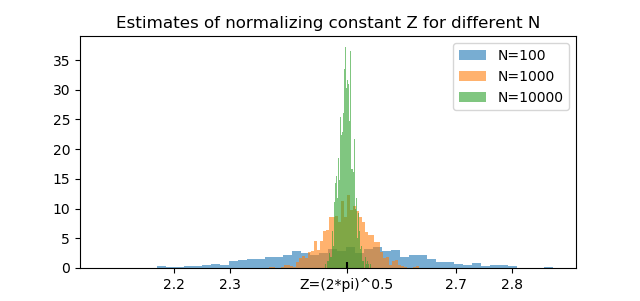
\includegraphics[width=0.7\linewidth]{1_b_hist_newg}
	\caption{For three different values of $N$ we see different variance in the estimate of Z. As $N$ increases, the variance decreases. The average of each histogram is close to the true value $Z=\sqrt{2\pi}$. The histogram was generated with 1000 simulations for each N.} 
	\label{fig:1bhist}
\end{figure}
The simulation results illustrated in figure \ref{fig:1bhist} demonstrates how the implemented IS is unbiased.

\paragraph{(c)} Now target the Cauchy distribution using the standard normal distribution.

\textbf{Solution: } The variance of the estimator is now
	\begin{equation}
		\int \dfrac{\pi^2(x)}{q(x)}dx - 1  = \int \dfrac{\gamma^2}{\pi^2(\gamma^2+x^2)^2}\dfrac{1}{\frac{1}{\sqrt{2\pi}}\exp\{-x^2/2\}}dx -1=\int \dfrac{\gamma^2}{\pi^2(\gamma^2+x^2)^2}\sqrt{2\pi}\exp\{x^2\}dx-1,
	\end{equation}
	which does not converge, i.e., the variance is infinite. Although the estimator is theoretically unbiased, it is numerically infeasible to attain an unbiased estimate.
	
%A problem arises here which is that the proposal explores a too small range of the target.
%The narrow exploration generates too many large weights, making the distribution of the estimate skewed.
%When $N$ increases, the estimated average approaches the true value $\pi$.
%
%If we increase the variance of the proposal from 1 to 20, giving it heavier tails the implementation clearly illustrates the unbiasedness even for $ N=100 $.
%%
Figure \ref{fig:1chist1} illustrates the IS with the standard normal distribution as proposal, and figure \ref{fig:1chist2} instead shows the histograms generated with the normal distribution with standard deviation 20 instead. An increased variance of the proposal decreases the bias that is actually implicitly introduced by this infinite variance.

\begin{figure}[t]
	\centering
	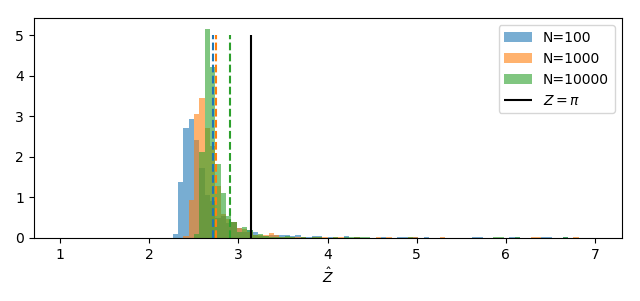
\includegraphics[width=.7\linewidth]{1_c_hist1}
	\caption{Task 1c. The distribution of the estimated normalization was skewed due to thin tails of the proposal.}
	\label{fig:1chist1}
\end{figure}
\begin{figure}[t]
	\centering
	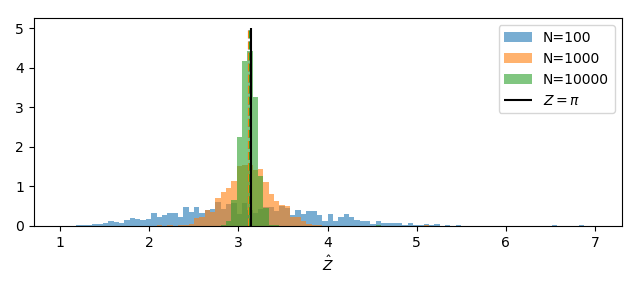
\includegraphics[width=.7\linewidth]{1_c_hist2}
	\caption{Task 1c. When the tails of the proposal were heavier, the estimates clearly clearly illustrated the unbiasedness of the IS.}
	\label{fig:1chist2}
\end{figure}




\cleardoublepage
\subsection*{H.2 Particle filter for a linear Gaussian state-space model}
\paragraph{(a)} The pdf's are $p(x_t|x_{t-1}) = \mathcal{N}(x_t; 0.8x_{t-1}, 0.5)$ and $ p(y_t|x_t) = \mathcal{N}(y_t;2x_t, 0.1) $.

\paragraph{(b)} Because we perfectly know the noise covariances, and that the model matches the simulated system, the Kalman filter is the optimal linear filter. The particle filter can on the other hand model nonlinearities in a model. But because our model is linear, we do not expect the particle filter trajectory to be closer to the true on average.

\paragraph{(c)} After implementing the bootstrap filter, the variance was computed for each $N$ as $Var(\hat{x}_t) = \sum_{i=1}^{N}w_t^i (x_t^i)^2 + \big(\sum_{i=1}^{N} w_t^i x_t^i \big)^2$. The Kalman filter's variance converges after only a few iterations. The variances are plotted in figure \ref{fig:2_c}.

Letting MAD denote the mean absolute difference between the BPF state estimate and the Kalman state estimate, averaged over time, the results together with average variance of the BPF is presented in table \ref{tab:2c}.
\begin{table}
	\caption{2c. Simulation results for the bootstrap particle filter. MAD is the mean absolute difference between the BPF estimated trajectory and the Kalman trajectory. The variance denotes the variance of the MAD over the iterations.}
	\label{tab:2c}
	\centering
	\begin{tabular}{lrr}\toprule
		$N$ & MAD 		& Variance 	\\\midrule
		10 	& 0.1489	& 0.020  	\\
		50	& 0.0412	& 0.023		\\
		100	& 0.0271	& 0.023		\\
		2000& 0.0060	& 0.024		\\
		5000& 0.0042 	& 0.024		\\
		Kalman & 0.0000 & 0.025		\\\bottomrule
	\end{tabular}
\end{table}

\begin{figure}[t]
	\centering
	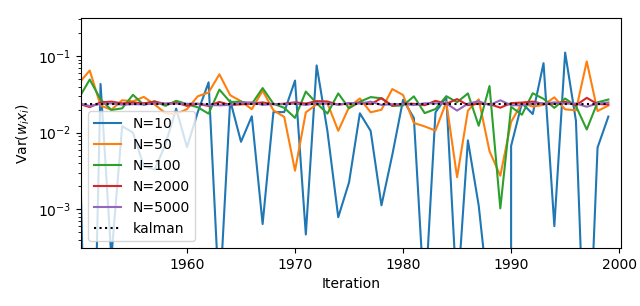
\includegraphics[width=.7\linewidth]{2_c}
	\caption{2c. Variance over particles per iteration of the BPF state estimates compared to the Kalman variance.}
	\label{fig:2_c}
\end{figure}

\paragraph{(d)} Derivation of the Fully Adapted Particle Filter pdf's follows.
The first proposal, for the adjustment multipliers $\bm{\nu}$:
	\begin{equation}
		\nu_{t-1}^i = p(y_t|x_{t-1}^i) = \dfrac{p(y_t,x_{t-1}^i)}{p(x_{t-1}^i)} \propto p(y_t,x_{t-1}^i).
	\end{equation}
	From the probabilistic model we have 
	\begin{equation}
		\mathcal{N}(y_t; 2x_t^i,0.1),
	\end{equation}
	from which we can plug in the model for $x_t^i$:
	\begin{equation}
		\mathcal{N}(y_t; 2(0.8x_{t-1}^i+V_t),0.1) = \mathcal{N}(y_t; 1.6x_{t-1}^i + 2V_t,0.1) = \mathcal{N}(y_t; 1.6x_{t-1}^i,2^2\cdot 0.5 + 0.1),
	\end{equation}
	thus, we have 
	\begin{equation}
		p(y_t|x_{t-1}^i) = \mathcal{N}(y_t; 1.6x_{t-1}^i, 2.1).
	\end{equation}
	
For the optimal proposal $q$:
	\begin{align}
		q(x_t|x_{t-1}, y_t) &\propto p(y_t|x_t,x_{t-1})p(x_t|x_{t-1}) = \mathcal{N}(y_t;2x_t,0.1)\mathcal{N}(x_t; 0.8x_{t.1},0.5) \propto\\
		&\propto \exp\{-\dfrac{(y_t-2x_t)^2}{2\cdot 0.1}\}\exp\{-\dfrac{(x_t-0.8x_{t-1})^2}{2\cdot 0.5}\}\propto\\
		&\propto\exp\{-\dfrac{(x_t-\frac{1}{42}(20y_t-1.6x_{t-1}))^2}{2\frac{1}{42}}\},
	\end{align}
so we get the normal distribution q:
	\begin{equation}
		q(x_t|x_{t-1}, y_t) = \mathcal{N}(x_t;~\frac{1}{42}(20y_t-1.6x_{t-1}), \frac{1}{42})
	\end{equation}


Table \ref{tab:2d} presents the MAD between the FAPF and the Kalman state trajectories for one simulation. Compared to the results for the BPF, the MAD is now a lot lower for small N, while they are still lower for larger N's but not as strikingly. 
	\begin{table}
		\centering
		\begin{tabular}{lr}\hline
			$N$ & MAD 		\\
			10 	& 0.0388	\\
			50	& 0.0181	\\
			100	& 0.0122	\\
			2000& 0.0028	\\
			5000& 0.0019 	\\
			Kalman & 0.0000	\\\hline
		\end{tabular}
		\caption{2d. The mean average difference between the Fully Adapted Particle filter's state trajectory and the Kalman filter's state trajectory.}
		\label{tab:2d}
	\end{table}

\paragraph{(e)} Figure \ref{fig:2_e} illustrates how only a few particles at time 1950 are remaining as ancestors for the final particles. 
	
	\begin{figure}[t]
		\centering
		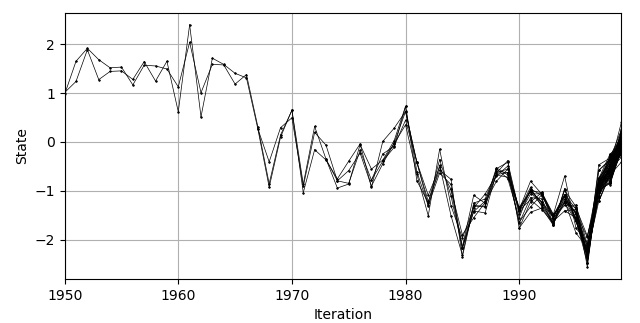
\includegraphics[width=.7\linewidth]{2_e}
		\caption{2e. Particle genealogy from time 1950 to 1999 for the fully adaptive particle filter. }
		\label{fig:2_e}
	\end{figure}

\paragraph{(f)} With systematic resampling the FAPF obtains less degeneracy and the final particles have many more ancestors. As illustrated in figure \ref{fig:2_f}, there are a lot more diversity in paths than in figure \ref{fig:2_e}. In figure \ref{fig:2_f_start} it is illustrated how the final 100 particles have 2-3 ancestors from the very beginning of the particle filter iteration.
	\begin{figure}[t]
		\centering
		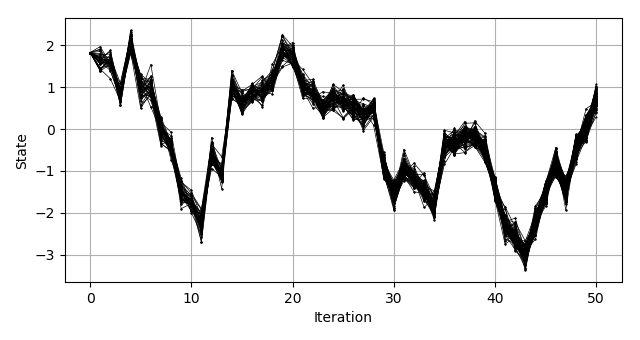
\includegraphics[width=.7\linewidth]{2_f}
		\caption{2f. The genealogy for the final 100 particles.}
		\label{fig:2_f}
	\end{figure}
	\begin{figure}[t]
		\centering
		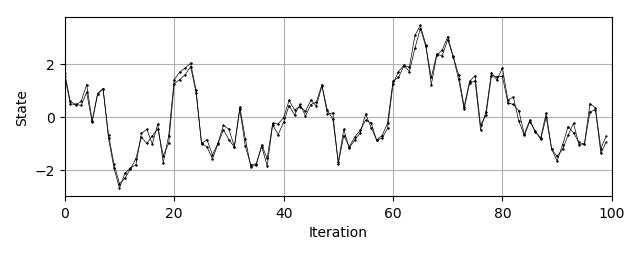
\includegraphics[width=.7\linewidth]{2_f_start}
		\caption{2f. The early genealogy for the final 100 particles.}
		\label{fig:2_f_start}
	\end{figure}

\paragraph{(g)}
For this task ESS triggered resampling was added to implementation.
With the threshold set to 50, resampling triggers around every 27:th iteration.
The path degeneracy became lower than in task 2f We can see that the amount of ancestors the final particles had in figure \ref{fig:2_g} is higher than in the results from 2f, in figure \ref{fig:2_f_start}.

\begin{figure}[h]
	\centering
	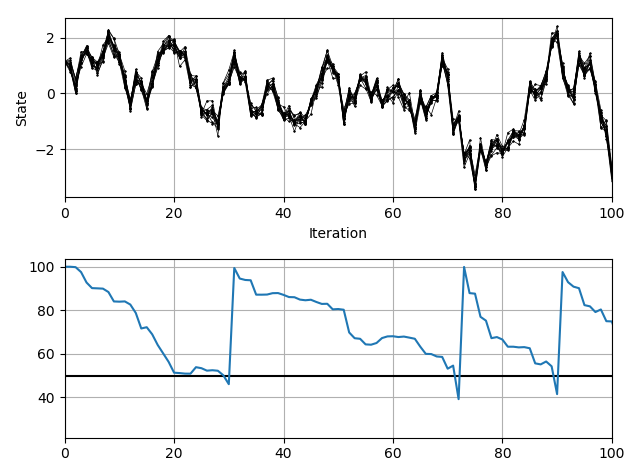
\includegraphics[width=.7\linewidth]{2_g}
	\caption{2g. (Top) The early genealogy for the final 100 particles using systematic resampling with ESS trigger at $ N_{\text{thresh}} = 50 $. (Bottom) The ESS in each iteration from 0 to 100.}
	\label{fig:2_g}
\end{figure}

\cleardoublepage
\section*{H.3 Parameter estimation in the stochastic volatility model}
\paragraph{(a)} Using a BPF with 100 particles, 10 estimates of the log-likelihood was created for the parameter $\phi$ on the range $ \{0.10, 0.15,\dots, 0.95, 0.96,\dots, 1.00\} $.
The results is presented as a boxplot in figure \ref{fig:3_a_new} and they indicate that phi around 0.96 gives the highest likelihood for the given data.
	\begin{figure}[t]
		\centering
		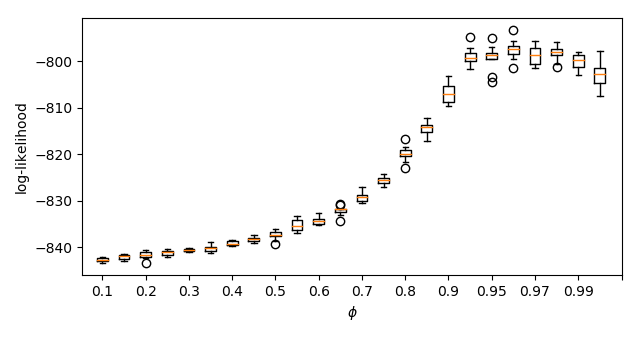
\includegraphics[width=\linewidth]{3_a_new}
		\caption{3a. Boxplot of the 10 log-likelihood estimates for each value of $\phi$. Note that the spacing of the phi-axis is smaller between 0.95 and 1, than it is before.}
		\label{fig:3_a_new}
	\end{figure}

\paragraph{(b)} The implementation for this exercise consisted of two main parts: the bootstrap particle filter (BPF) to return the log-likelihood, and the particle Metropolis-Hastings (PMH) algorithm to iterate over parameters proposals.
In the BPF, the unnormalized logarithmic weights $\tilde{v}_t$ are computed as
	\begin{equation}
		\tilde{v}_t^i = \ln\dfrac{1}{\sqrt{2\pi\beta^2\exp\{x^i_t\}}} - y_t^2,~i=1,\dots, N.
	\end{equation}
Then their maximum is subtracted to get the shifted log-weights $v_t^i$:
	\begin{equation}
		v_t^i = \tilde{v}_t^i - \max_i \tilde{v}_t^i.
	\end{equation}
The log-likelihood is then computed as
	\begin{equation}
		z_t = \max_i \tilde{v}_t^i - \ln N + \ln\sum_{i=1}^{N}\exp\{v_t^i\},
	\end{equation}
so that the total log-likelihood $Z$ for the PMH iteration was the sum over $z_t$ over all $t=1,\dots, T$:
	\begin{equation}
		Z = \sum_{t=1}^{T} z_t.
	\end{equation}
The resampling weights $w_t^i$ are then computed as 
	\begin{equation}
		w_t^i = \dfrac{\exp\{v_t^i\}}{\sum_{t=1}^T\exp\{v_t^i\}}.
	\end{equation}

The implementation computes the acceptance probabilities by the logarithms of the fraction for $\alpha$ as described in the lecture, by summing the log-likhelihoods $Z'$ for the proposed parameters $\beta', \sigma'$, and $Z$ for the previous parameters $\beta, \sigma$:
	\begin{equation}
		\alpha = \min\{ 1, \exp\{\alpha_1' - \alpha_1\}\},
	\end{equation}
	\begin{equation}
		\alpha_1' = Z' + \ln(\mathcal{IG}(\beta', 0.01, 0.01)) + \ln(\mathcal{IG}(\sigma', 0.01, 0.01)),
	\end{equation}
	\begin{equation}
		\alpha_1 = Z + \ln(\mathcal{IG}(\beta, 0.01, 0.01)) + \ln(\mathcal{IG}(\sigma, 0.01, 0.01)).
	\end{equation}

The step size $\mu$ for the Gaussian random walk was set to 0.01 for both $ \beta $ and $ \sigma $, the number of PMH iterations to $M=10000$ with $N=1000$ particles while the initialization was set to 0.5 for both variables. The Gaussian random walk is performed on the non-squared parameters, so $\beta', \sigma' \sim \mathcal{N}(0, 0.01^2)$.

With these settings the plots in figure \ref{fig:3_b} were generated.
There is seemingly a large bump in the evolution for $\beta^2$ between iteration 3000 and 5000.
This might be part of the burn-in, but yet they are included in the histogram.
\begin{figure}[h]
	\centering
	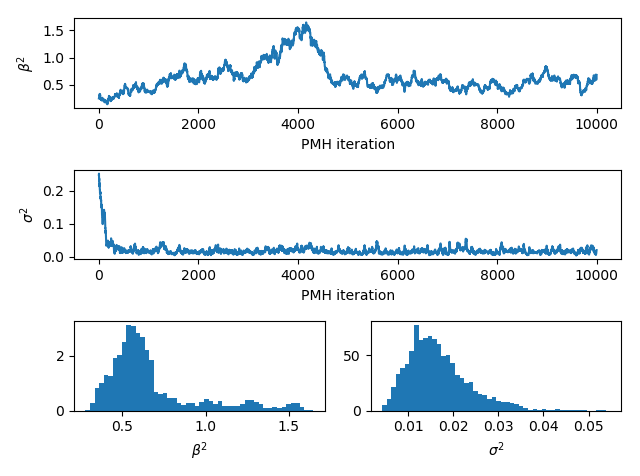
\includegraphics[width=0.7\linewidth]{3_b}
	\caption{3b. (Top and middle) The evolution of $\beta^2$ and $ \sigma^2 $ over the PMH iterations. (Bottom) Histograms of the parameters over the last 8000 iterations.}
	\label{fig:3_b}
\end{figure}

\paragraph{(c)} The particle Gibbs algorithm requires samples from the inverse Gamma distribution, which was implemented as inverting the sample from the gamma distribution in numpy: \texttt{1/numpy.random.gamma(a, 1/b)} where \texttt{a, b} are the parameters as described in the homework information.

There was some problems in generating results from the particle Gibbs algorithm using the implementation. Some problem with the evolution of the $b$ parameter for $\beta$ makes it explode, and the sampling from the inverse Gamma distributions returns very large values on $\beta$ and the algorithm breaks down. As stated in the instructions, the particle Gibbs and the PMH are consistent MCMC samplers, and should therefore return the same posterior distributions. I cannot seem to find the issue with my implementation


\cleardoublepage
\section*{H.4} The annealing sequence was designed as 

	\begin{equation}
		\pi_k(x) = \bm{1}_{0\leq x_1\leq 1}\bm{1}_{0\leq x_2\leq 1}\Big(\cos^2(\pi x_1)\sin^6(3\pi x_2)\exp(-30(x_1^2+x_2^2))\Big)^{k/K}
	\end{equation}
	so that we can sample from $ \pi_0(x) = \mathcal{U}(x: 0, 1) $ where both components $x_1, x_2$ are uniformly distributed between 0 and 1.
	
	The presented results were generated with parameters set as $ K=80 $, $ N=100 $, $0.02$ standard deviation for the Gaussian random walk and ESS triggered resampling at $N_{\text{thresh}}= 70$.
	
	The particles at four different iterations are shown in figure \ref{fig:4_a}, and the $N_\text{eff}(k)$ in \ref{fig:4_b}. The estimate of normalizing constant was $\hat{Z}=6.84$.
	
	The average consecutive iterations between resampling was 10. For different seeds in the simulation, this number would vary within the range from 10 to 16.

\begin{figure}[h]
	\centering
	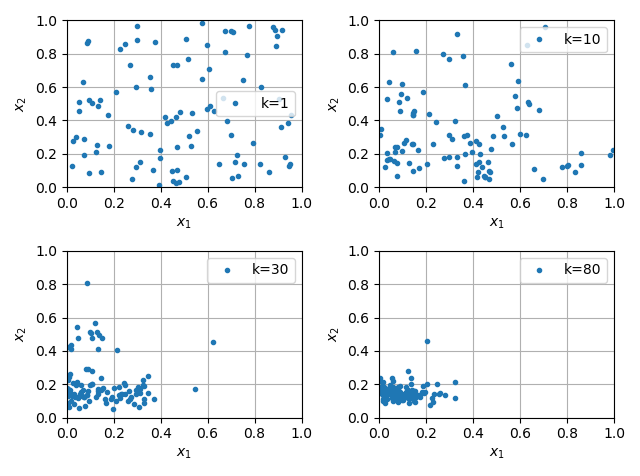
\includegraphics[width=.7\linewidth]{4_a}
	\caption{4a. (Top left) The particles at initialization were sampled from the standard uniform distribution. (Top right) The particles after 10 iterations had all been moved into several clusters. (Bottom left) The particles after 30 iterations were a lot more concentrated on $x_2=0.15$ while more spread out for $x_1$, some sinusoidal effect is seen over $x_2$ having a cluster between 0.4 and 0.6. (Bottom right) After 80 iterations almost no effect of the sinusoidal functions were visible as they were more overshadowed by the exponential.}
	\label{fig:4_a}
\end{figure}
\begin{figure}[h]
	\centering
	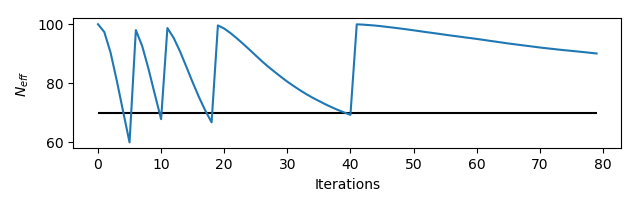
\includegraphics[width=.7\linewidth]{4_b}
	\caption{4b. The number of iterations between resampling is increasing with the iteration number, while the average for these 150 iterations is 19. }
	\label{fig:4_b}
\end{figure}
\end{document}	